





%%
%% The "title" command has an optional parameter,
%% allowing the author to define a "short title" to be used in page headers.
\chapter{GPU-acceleration of neighborhood-based dimensionality reduction algorithm EmbedSOM}

%%
%% The "author" command and its associated commands are used to define
%% the authors and their affiliations.
%% Of note is the shared affiliation of the first two authors, and the
%% "authornote" and "authornotemark" commands
%% used to denote shared contribution to the research.
% \author{Adam Šmelko}
% \email{smelko@d3s.mff.cuni.cz}
% \orcid{0000-0001-8334-2783}
% \author{Martin Kruliš}
% \email{krulis@d3s.mff.cuni.cz}
% \orcid{0000-0002-0985-8949}
% \author{Jiří Klepl}
% \email{klepl@d3s.mff.cuni.cz}
% \orcid{0000-0002-2231-4073}
% \affiliation{%
%   \institution{Department of Distributed and Dependable Systems, Charles University}
%   \city{Prague}
%   \country{Czechia}
% }


% \keywords{Dimensionality reduction, Single-cell cytometry, GPU acceleration, CUDA, kNN, Optimizations}


\section{Introduction\label{sec:intro}}

Dimensionality reduction algorithms emerged as indispensable utilities that enable various forms of intuitive data visualization, providing insight that in turn simplifies rigorous data analysis.
The development has benefited especially the life sciences, where algorithms like t-SNE~\cite{maaten2008visualizing} reshaped the accepted ways of interpreting many kinds of measurements, such as genes, single-cell phenotypes and development pathways, and behavioral patterns~\cite{toghi2019quantitative,cande2018optogenetic}.

The performance of the non-linear dimensionality reduction algorithms becomes a concern if the analysis pipeline is required to scale or when the results are required in a limited amount of time such as in clinical settings.
To tackle the limitations of poor scalability, Kratochvíl et al. developed EmbedSOM~\cite{kratochvil2019generalized}, a dimensionality reduction and visualization algorithm based on self-organizing maps (SOMs)~\cite{kohonen1990self}.
EmbedSOM provided a $10\times$ speedup on datasets typical for single-cell cytometry data visualization while retaining the competitive quality of the results.
Still, the parallelization potential of EmbedSOM remained mostly untapped as of yet.

This paper describes an efficient, highly parallel GPU implementation of EmbedSOM designed to provide real-time results on large datasets. The implementation is accompanied by performance benchmarks of individual optimizations to evaluate the optimal variants for different dataset sizes. Both the implementation and the empirical data are available in our GitHub repository\footnote{\url{https://github.com/asmelko/gpgpu24-artifact}}.

In the paper, we first describe the EmbedSOM algorithm in Section~\ref{sec:methods}. We specifically detail the CUDA-based GPU implementation of the algorithm in Section~\ref{sec:impl} and evaluate its performance in Section~\ref{sec:results}. Related work is discussed in Section~\ref{sec:embedsom_relwork} and Section~\ref{sec:outro} concludes the paper.

% Dimensionality reduction algorithms emerged as indispensable utilities that enable various forms of intuitive data visualization, providing insight that in turn simplifies rigorous data analysis.
% Various algorithms have been proposed for graphs and high-dimensional point-cloud data, and many different types of datasets that can be represented with a graph structure or embedded into vector spaces.
% The development has benefited especially the life sciences, where algorithms like t-SNE~\cite{maaten2008visualizing} reshaped the accepted ways of interpreting many kinds of measurements, such as genes, single-cell phenotypes and development pathways, and behavioral patterns~\cite{toghi2019quantitative,cande2018optogenetic}.

% The performance of the non-linear dimensionality reduction algorithms becomes a concern if the analysis pipeline is required to scale or when the results are required in a limited amount of time such as in clinical settings.
% The most popular methods, typically based on neighborhood embedding computed by stochastic descent, force-based layouting or neural autoencoders, reach applicability limits when the dataset size is too large.
% To tackle the limitations, we have previously developed EmbedSOM~\cite{kratochvil2019generalized}, a dimensionality reduction and visualization algorithm based on self-organizing maps (SOMs)~\cite{kohonen1990self}.
% EmbedSOM provided an order-of-magnitude speedup on datasets typical for single-cell cytometry data visualization while retaining the competitive quality of the results.
% The concept has proven useful for interactive and high-performance workflows in cytometry~\cite{kratochvil2020shinysom,kratochvil2020gigasom}, and easily applies to many other types of datasets.
% Despite that, the parallelization potential of the extremely data-regular design of EmbedSOM algorithm has remained mostly untapped.

% Our contribution in this paper is a natural continuation of the development:
% We describe an efficient, highly parallel GPU implementation of EmbedSOM designed to provide interactive results on large datasets.
% The implementation is sufficiently fast to provide real-time visualizations of datasets larger than $10^5$ of individual data points on off-the-shelf hardware, while maintaining smooth video-like frame rate.
% We demonstrate that the result gives unprecedented, controllable view of the details of specific high-dimensional datasets.
% The instant feedback available to the user opens possibilities for partial supervision of the visualization process, allowing user-intuitive resolution of possible visualization ambiguities as well as natural exploration of new datasets.
% We demonstrate some of the achievable results on two realistic datasets.
% The resulting software, called \emph{BlosSOM}, is published as free and open source.
% BlosSOM can be readily utilized to reproduce our results and explore more datasets; additionally it contains support for working with data formats (mainly, the FCS standard~\cite{fcs}) that make it immediately useful for visualization of existing and new biological data.

% In the paper, we briefly describe the EmbedSOM algorithm (Section~\ref{ssec:embedsom}), and show an extension of its generalized form that dynamically mixes the user feedback to the learning process, thus enabling the semi-supervised learning (Section~\ref{ssec:dynamic}).
% We specifically detail the CUDA-based GPU implementation of the algorithm in Section~\ref{sec:impl}, and report the achieved performance improvements (Section~\ref{ssec:perf}).
% Finally, we showcase the achievable results on biological data, and discuss possible future enhancements and applications that would aid data analysis (Sections~\ref{ssec:appl}, \ref{ssec:future}).

\section{Landmark-directed dimensionality reduction\label{sec:methods}}

EmbedSOM is a visualization-oriented method of non-linear dimensionality reduction that works by describing a high-dimensional point by its location relative to landmarks equipped with a topology and reproducing the point in a low-dimensional space using an explicit low-dimensional projection of the landmarks with the same topology~\cite{kratochvil2019generalized}.
% The ability to effectively work with a simplified model of the data differentiates it from other dimensionality reduction methods; in turn it offers superior performance by reducing the amount of necessary computation as well as by opening parallelization potential, since the computations of the projections of many individual points are independent.
% In the setting of flow and mass cytometry data visualization, this provided speedup of several orders of magnitude against the other available methods~\cite{kratochvil2020gigasom,kratochvil2020shinysom}.

% While the EmbedSOM originally used the (eponymous) self-organizing maps to find the viable high- and low-dimensional manifolds from the data points, the concept generalized well to many other methods.
% In particular, the projection has been shown to work with any (even random) set of high-dimensional landmarks that have the low-dimensional counterparts organized by any selected dimensionality reduction method (which may be slow in comparison, given the fact that the set of landmarks is usually small).
% In Section~\ref{ssec:dynamic}, we utilize this freedom of model specification to provide dynamic view of the dataset, based on a simplified dataset model that the user may refines in order to improve the dataset view.

More formally, the EmbedSOM algorithm works as follows. Let $d$ be the dimension of the high-dimensional space and assume $\mathbb{R}^2$ is the low-dimensional space for brevity. EmbedSOM processes $n$ $d$-dimensional points in a matrix $X$ of size $n\times d$, and outputs $n$ 2-dimensional points in matrix $x$ of size $n\times 2$.
The high- and low-dimensional landmarks similarly form matrices $L$ of size $g\times d$ and $l$ of size $g\times 2$, where usually $g\ll n$.
Each point $X_i$ is transformed to a point $x_i$ as:
\begin{enumerate}
\item $k$ nearest landmarks are found for point $X_i$ ($k$ is a constant parameter satisfying $3\leq k\leq g$)
\item the landmarks are ordered and a score is assigned to each of them, using a smooth function of the distance that assigns the highest score to the closest landmark and $0$ to the $k$-th landmark (this ensures the smoothness of projection in cases when $k<g$ \cite{kratochvil2019generalized})
\item for each pair $(u,v)$ of the closest $k-1$ landmarks (i.e., the ones with non-zero score), a projection of the point $X_i$ is found on the 1-dimensional affine space with coordinate 0 at $L_u$ and 1 at $L_v$; the 1-dimensional coordinate of the projection in this affine space is taken as $D_{uv}(X_i)$ and the same projected coordinates are defined in the low-dimensional space as $d_{uv}(x_i)$
\item point $x_i$ is fitted to the low-dimensional space so that the squared error in the coordinates weighed by nearest-landmark scores ($s_u, s_v$) is minimized: $$x_i = \argmin_{p\in \mathbb{R}^2} \sum_{u,v}s_u\cdot s_v\cdot \left(D_{uv}(X_i)-d_{uv}(p)\right)^2$$
\end{enumerate}

Because $d_{uv}(p)$ is designed as a linear operator, the error minimization problem (step 4) collapses to a trivial solution of $2$ linear equations with $2$ variables.
A complete algorithm may be found in the original publication~\cite[Algorithm 1]{kratochvil2019generalized}.

% Efficient implementation of the EmbedSOM algorithm is the main performance concern that enables its interactive use.
% The original CPU-based parallel implementation was able to visualize hundreds of thousands of points per second on common use-cases.
% As a major result of this paper, in Section~\ref{sec:impl} we improve this performance to the scale of milliseconds, enabling real-time projection and rendering of points based on interactive control of the high- and low-dimensional landmarks.

% \subsection{User supervision and model interaction}
% \label{ssec:dynamic}

% EmbedSOM landmarks (the matrices $L$ and $l$) represent a simplified dataset model that can be used to conveniently and predictably steer the dimensionality reduction.
% In particular, the main property of the projection --- visualizing the data points from the neighborhood of a landmark $L_i$ preferably in the neighborhood of the corresponding low-dimensional $l_i$ --- gives an intuitive interpretation for the landmark positions:
% Manipulating the high-dimensional landmarks chooses which data are visualized, while manipulating the low-dimensional landmarks chooses the desired location of the visualized points.
% Smoothness of the projection then grants that the smooth manipulations of the landmarks that will result in smooth changes of the results, enabling predictable user control and refinement.

% However, positioning of the landmarks in the high-dimensional space (which is inherently complicated to navigate) and finding a suitable layout of the landmarks in the low-dimensional space is an overly complicated task for the user alone.
% The main concern of this section is to design a simplification of the control of the landmarks, so that viable results may be reached in an automated way and the user interaction is required only for decisions that can not be decided automatically such as resolving dimensionality-reduction ambiguities and positioning of the dataset parts that matches some assumed semantics.
% We describe two ways of automated and user-controlled positioning of the landmarks that implement this kind of partial supervision, thus making the method semi-supervised.
% Both are roughly based on the embedding methods proposed in previous work~\cite{kratochvil2019generalized}; only modified for interactive environment.

% The main tasks that the user supervision interface has to resolve are thus as follows:
% \begin{itemize}
% \item place the landmarks to viable positions in the high-dimensional space
% \item dynamically increase or decrease the resolution of the model in specified places, by adding or removing landmarks
% \item organize low-dimensional landmarks to reflect the structure in the high-dimensional space, while allowing the user to resolve ambiguities that arise in dimensionality reduction
% \item react to the changes in the input datasets, such as scaling of the dimensions and appearance of new points
% \end{itemize}

% \begin{figure}
% \centering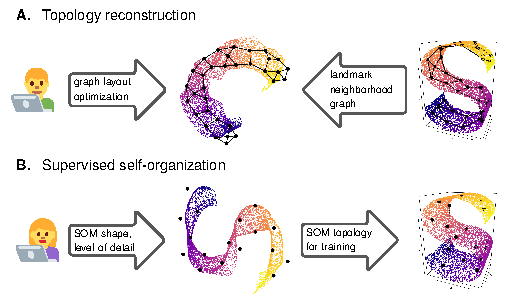
\includegraphics[width=\linewidth]{embedsom/pic/sup.pdf}
% \caption{
% Schema of the 2 implemented user supervision approaches.
% The user interacts with low-dimensional model that is intuitive to navigate, and indirectly drives the positioning of the corresponding high-dimensional image of the model, using either a graph-based approach (Section~\ref{sssec:sup-graph}) or self-organizing map approach (Section~\ref{sssec:sup-som}).
% }
% \label{fig:supervis}
% \end{figure}

% The two methods detailed below are briefly illustrated in Figure~\ref{fig:supervis}.

% \subsubsection{Semi-supervised structure reconstruction}
% \label{sssec:sup-graph}

% One possible approach to position the high-dimensional landmarks is to sample them randomly from the distribution of the original data set, and position the low-dimensional ones to reflect the structure of the sampling.
% In the original unsupervised implementation, we used a random sample of the input dataset as the landmark positions, and a dimensionality reduction methods such as t-SNE to position the landmarks.
% Importantly, the positioning of low-dimensional landmarks could be performed relatively quickly even by rather time-demanding algorithms such as t-SNE, because the algorithm only had to work with the highly reduced version of the dataset in landmarks.

% In the dynamic, supervised context, we need to avoid the randomness in order to avoid flickering in the view of the dataset, and utilize a dimensionality reduction algorithm that may reflect the user input.
% Thus, we chose to continuously run an interactive version of $k$-means clustering with a low learning rate to find good $k$ high-dimensional landmarks $L$, and employ a simple force-based graph layouting algorithm on a neighborhood graph of $L$ to embed the landmarks to 2D.
% Both these algorithms are capable of smooth transitions between consecutive states, thus avoiding the flicker.
% Moreover, force-based graph layouting may be intuitively steered by the user by dragging the graph nodes. Similarly, the points may be added and removed from $k$-means clustering in the same interface in order to increase and decrease the model resolution.

% Addition of a new landmark is implemented as follows: The user selects a low-dimensional landmark, and upon pressing a special button, both the low-dimensional landmark and its high-dimensional counterparts are duplicated in their respective spaces.
% The $k$-means algorithm then consecutively optimizes the positions of the landmarks to provide a detailed view.
% This stability of the result is helped by the initialization properties of $k$-means where the cluster centroids tend to stay in the same clusters~\cite{franti2019much} (counter-intuitively, the same properties have an undesirable impact on the robustness of unsupervised clustering).
% Most importantly, this enables the user to position new landmarks without having to navigate the possibly overwhelming complexity of the data distribution in the high-dimensional space.

% \subsubsection{Supervised training of self-organizing maps}
% \label{sssec:sup-som}

% Alternatively, the user may choose a SOM approach as originally intended for EmbedSOM.
% BlosSOM supports user drawing of the 2-dimensional version of the SOM on a canvas, which is used as-is as the low-dimensional landmarks.
% New landmarks may be added at any position, as their initial high-dimensional coordinates can be fitted using the coordinates of the other close landmarks in 2D.

% The positioning of the landmarks in 2D is then used as a topology for training the high-dimensional landmarks as neuron weights of the SOM algorithm.
% To extend the supervision possibilities of this step, BlosSOM adds specific controls that allow the user to manually sweep through the SOM neighborhood sizes and learning rates (usually labeled $\sigma$ and $\alpha$ \cite{kohonen1990self}), which is done automatically in unsupervised SOM training.
% This allows the users to optionally pause the SOM training at any stage and fix or customize the SOM topology at coarse detail level (with larger $\sigma$) before it is used to train fine details (small $\sigma$, the difference is closer detailed in Figure~\ref{fig:somsigma}).

% \begin{figure}
% \centering
% \begin{tikzpicture}[node distance=1em]
% \node (a) {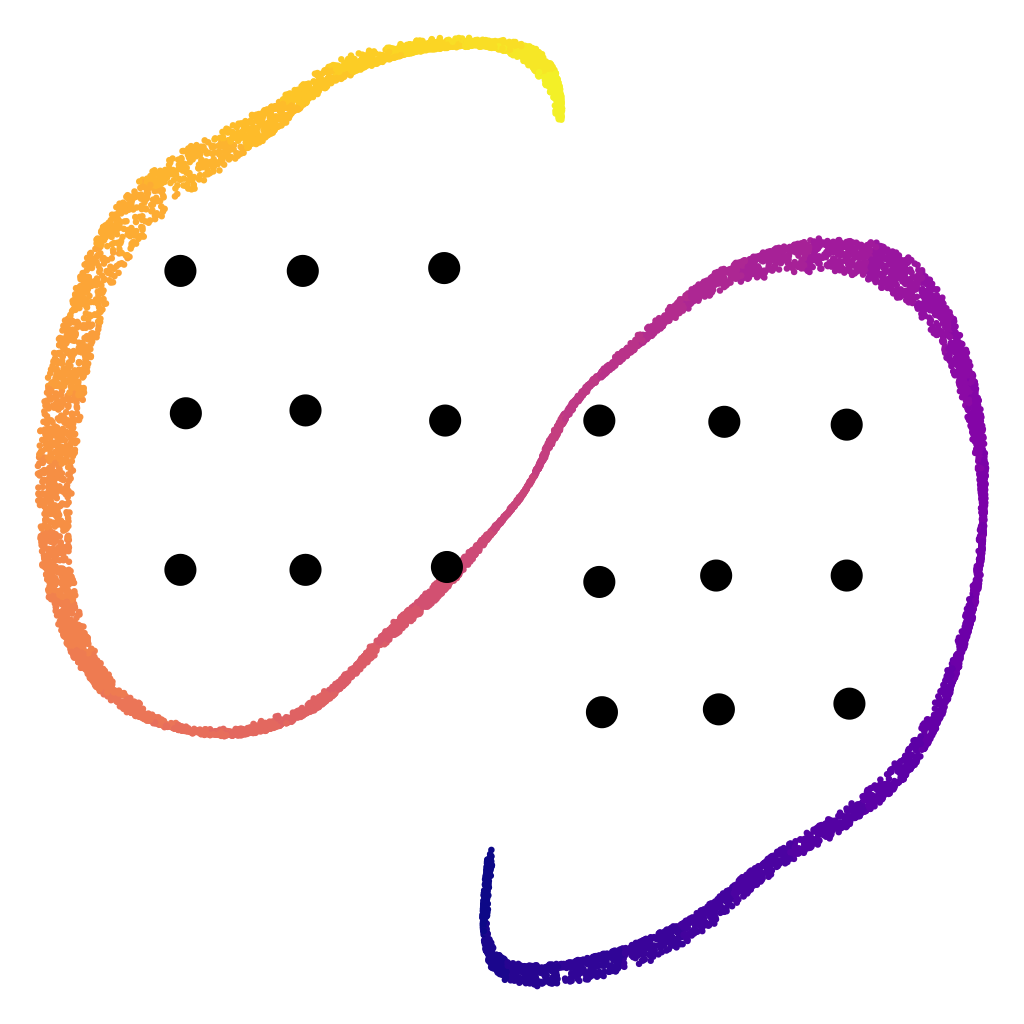
\includegraphics[width=.25\linewidth]{embedsom/pic/S_begin_2d.png}};
% \node[right=of a] (b) {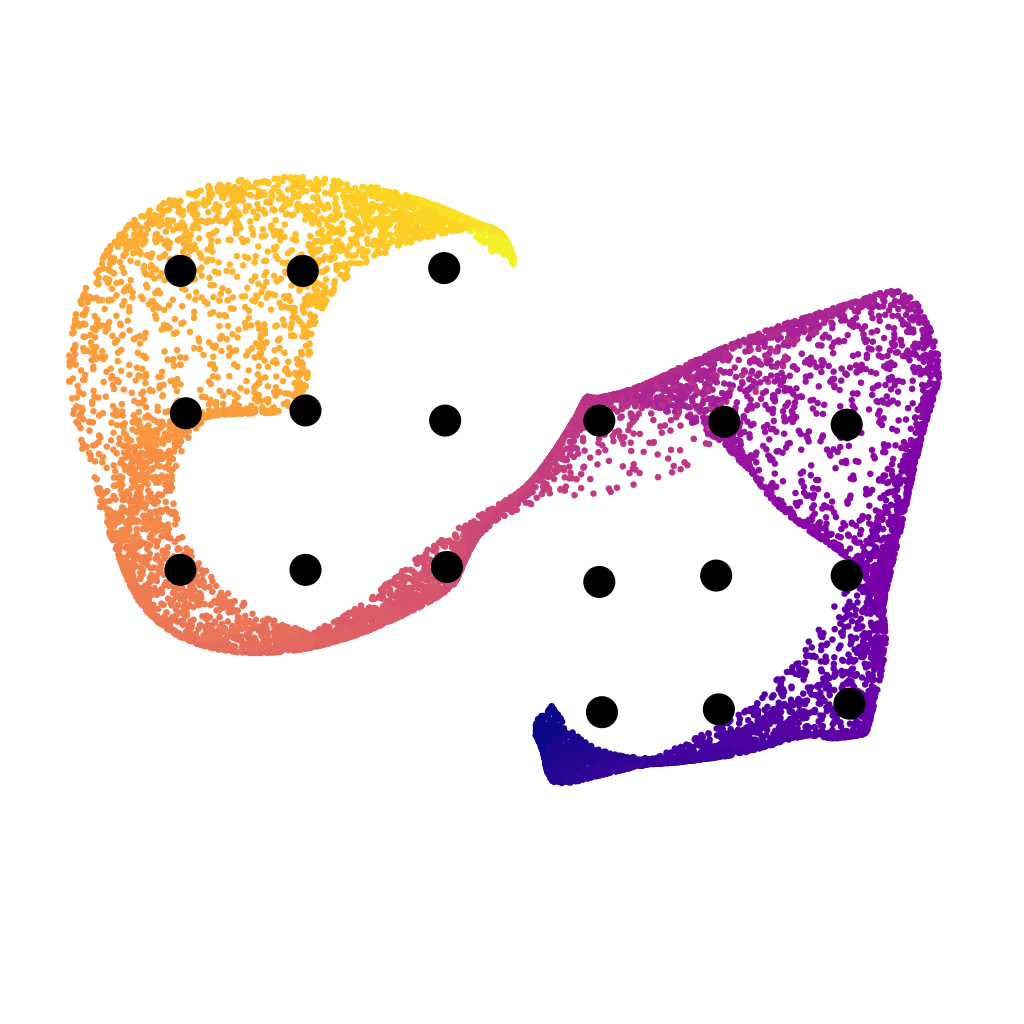
\includegraphics[width=.25\linewidth]{embedsom/pic/S_mid_2d.png}};
% \node[right=of b] (c) {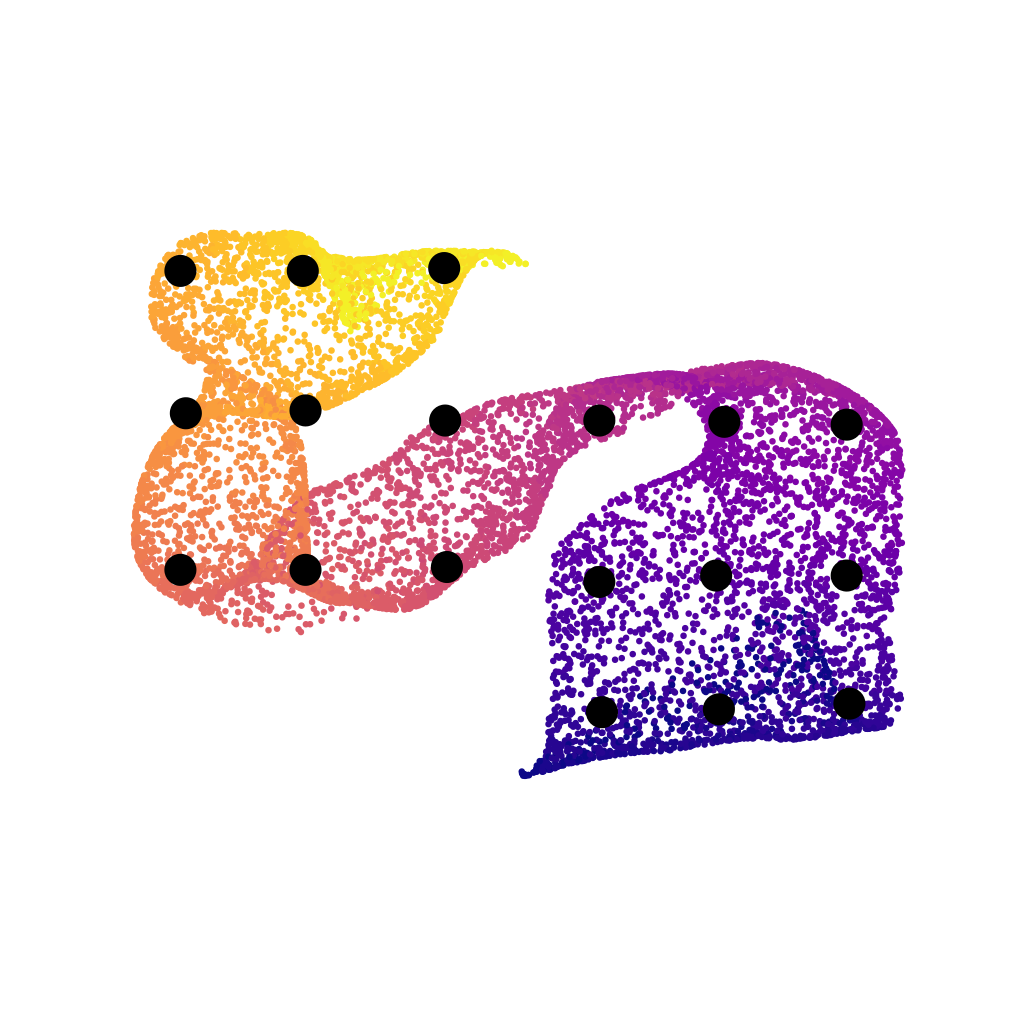
\includegraphics[width=.25\linewidth]{embedsom/pic/S_end_2d.png}};
% \node[below=0pt of a] {$\sigma=1.5$};
% \node[below=0pt of b] {$\sigma=0.8$};
% \node[below=0pt of c] {$\sigma=0.2$};
% \end{tikzpicture}
% \caption{
% Effect of different settings of $\sigma$ SOM training parameter on the output detail, demonstrated on an extruded S-shaped 3D dataset and a custom SOM shape.
% Value of $\sigma$ decreases from left to right, progressively revealing finer details but losing larger-scale structure.
% }
% \label{fig:somsigma}
% \end{figure}

\section{GPU implementation of EmbedSOM}\label{sec:impl}

While EmbedSOM is relatively straightforward to parallelize for mainstream CPU architectures, several challenges appear when designing of an optimal implementation for contemporary GPUs.
In this section, we outline the key optimizations that allowed us to run the high-performance dimensionality reduction in EmbedSOM, and give an overview of the relative performance gains achieved by the algorithm choice.

Technically, the algorithm consists of two main parts that provide distinct implementation challenges:

\begin{itemize}
\item {\bfseries $k$-NN step}\quad
The search of $k$-nearest landmarks in $L$ for each data point from $X$ requires a highly irregular selection of indices of $k$ lowest values from columns of the dynamically computed distance matrix $L^T\cdot X$.

\item {\bfseries Projection step}\quad
Computation of the small linear system that is used to find the minimal-error-projection of a point, namely of projections $D_{uv}$ and the derivatives $\frac{\delta d_{uv}}{\delta x_i}$ (Section~\ref{sec:methods}), is difficult to optimize due to irregular memory access patterns of collecting the data for the computation.
\end{itemize}

% We carried out the implementation in NVIDIA CUDA~\cite{guide2013cuda}, the performance validation presented in the next sections is accordingly carried out only on NVIDIA hardware that supports CUDA.
% Despite our benchmarks being NVIDIA-specific, the presented kernels do not depend on any NVIDIA-specific functionality, and the results should be portable to other GPU programming frameworks (such as Vulkan Compute shaders) and hardware of other vendors.
% We expect that only minor adjustments will be required to compensate for GPU design differences, such as the 64-thread wavefronts on AMD devices.

In the following two sections, we describe in detail the optimizations of the CUDA implementation.

\subsection{$k$-NN selection step}\label{sec:impl-knn}

The task of the first part of the algorithm is to find $k$ nearest landmarks (from $L$) for every data point in $X$.
This comprises two sub-steps: computing Euclidean distances for every pair from $L$ and $X$ and performing point-wise reduction that selects a set of $k$ nearest landmarks for each of the $n$ points, based on the computed distances.

While the Euclidean distance computation is mathematically simple and embarrassingly parallel, achieving optimal throughput on GPUs is quite challenging~\cite{krulivs2017employing}.
In particular, the ratio between the data transfers and the arithmetic operations performed by each GPU core is heavily biased towards data transfers.
The overhead of data transfers is best prevented by finding a good caching pattern for the input data that is able to optimally utilize all hardware caches (L1 and L2), shared memory, and core registers.

The parallel implementation of the $k$-nearest neighbors search is even more challenging.
The $k$-NN problem is computed individually for each data point, which provides the space for possible parallelization.
However, concurrently processed instances of a na\"{i}ve $k$-NN implementation exhibit severe code divergence because the selection process is purely data-driven, and requires a high amount of memory allocated per core.
Optimally, the $k$-NN selection is realized by customized versions of parallel sorting algorithms, which are well-researched and possess existing GPU implementations~\cite{singh2018survey}.

Our implementation chooses to optimize both sub-steps since the ratio of the amount of required computations can be easily biased by the configuration of parameters $d$ and $k$.
In particular, processing high-dimensional datasets with a low $k$ parameter spends significantly more time in the distance computation, but lower-dimensional datasets with higher $k$ require more time in the nearest neighbor selection.

Concerning the perspective of software design, the implementation may use separate kernels for both sub-tasks or a single fused kernel.
Kernel separation provides better code modularity and much flexibility in work-to-thread division and data caching strategy, at the cost of having to materialize all the computed distances in the GPU global memory, thus significantly increasing the total amount of data transfers.
Contrary to that, a fused kernel may immediately utilize the computed distances in $k$-NN computation without transferring the data to global memory and interleaving the distance computations with $k$-NN may help to improve the ratio between computations and data transfers.
Since our initial observations showed that the overhead of the data transfers required for kernel communication is relatively high, we decided to implement only the fused variant for the sake of simplicity.
The usage of separate kernels might be interesting in the future, especially for extreme values of $d$ that diminish the relative cost of the distance data transfer.

\subsubsection{Available algorithms for $k$-NN}

There are many approaches to $k$-NN selection, varying in complexity and parameter-dependent performance. We implemented several of the possibilities (as described in this section) to substantiate our choice of the algorithm for GPU EmbedSOM.

As a baseline (labeled \Alg{Base}), we used the most straightforward approach to GPU parallelization which simply invokes original sequential code for every data point concurrently.
The \alg{Base} kernel is spawned in $n$ threads (one for each data point), and each thread computes the distance between its data point and all landmarks while maintaining an ordered array of $k$ nearest neighbors.
The array is updated by an insert-sort step performed for every new computed distance --- i.e., by starting at the end of the array and moving the new distance-index pair towards smaller values until it reaches the correct position.

\Alg{Shared} algorithm is a modified version of the baseline algorithm that utilizes shared memory as a cache, following the recommended optimization practice of improving performance by caching data that are reused multiple times~\cite{guide2013cuda}.
In this case, we cache the landmark coordinates, which are sufficiently small to fit in the shared memory for all tested parametrizations.

In \Alg{GridInsert} algorithm, we utilize the shared memory to cache both landmarks and points.
However, the limited size of shared memory imposes limitations of the amount of cached data. Hence, the algorithm was parametrized by the block height $h$ (number of cached points from $X$) and the block width $w$ (number of cached landmarks from $L$).
The algorithm runs in epochs, each of which first caches $h$ points and $w$ landmarks, and then computes $h \cdot w$ distance values using only data in shared memory.
While the distances are computed concurrently by the whole thread block, we chose to avoid explicit synchronization in the $k$-NN step, using only $h$ threads to incorporate the newly computed distances into $h$ separate $k$-NN results using the insert-sort steps.
The \alg{GridInsert} should achieve better throughput in the distance computation thanks to the caching, at the cost of slightly sub-optimal $k$-NN reduction; thus, giving the best performance on high-dimensional datasets and low values of $k$.

% The above algorithms focus solely on optimizing the distance computation; we further detail the possible optimizations of the $k$-NN selection.

% A straightforward way for computing the $k$ nearest neighbors in parallel is to sort an entire array of distances using a parallel sorting algorithm, then taking the first $k$ items.
% Although the overhead of storing the distances might be excessive, we expected the strategy to be competitive especially for large values of $k$ (approaching the total number of landmarks in the grid).
% We use this approach in \Alg{Radix} algorithm, which employs the highly-optimized sorting algorithm from the state-of-art CUB library~\cite{cub}.
% The algorithm allocates an entire thread block to process one input data point.
% The block cooperates on computing the Euclidean distances by dividing the landmarks evenly among the threads.
% The distances are stored along with indices in the shared memory block, which is then sorted by the CUB radix sort, and subsequently the first $k$ items are copied to the result buffer in global memory.
% Importantly, the whole block of $g$ distance-index pairs must fit in the shared memory, which imposes a limitation on the maximal amount of landmarks, and prevents much of the input caching in the shared memory, impacting the efficiency of distance computation.

Finally, improvising on our previous work~\cite{krulivs2015optimizing}, we implemented \Alg{Bitonic} $k$-NN selection algorithm, which utilizes routines from the highly parallelizable bitonic sorting algorithm.
Bitonic sorting is very suitable for parallel lockstep execution~\cite{krulivs2017employing}, and the capability to merge sorted sequences has allowed us to keep only $2k$ distances (instead of $g$) in the shared memory.
This method benchmarked the best on the average, so it is selected as default for EmbedSOM and we describe it more thoroughly in the following.


\subsubsection{Bitonic approach to $k$-NN}

The \alg{Bitonic} approach can be seen as a combination of the benefits of the other algorithms: It does not require materializing all distances in the memory to do a full sort and even though it does not use an elaborate input caching strategy like \alg{GridInsert}, it still gives interesting results because the data loading operations can be partially overlapped with bitonic sorting operations if enough warps are allocated to one streaming multiprocessor.

\begin{figure}
	\centering
	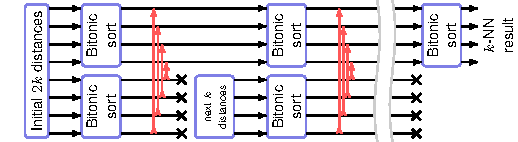
\includegraphics{embedsom/pic/bitonic.pdf}
	\caption{\alg{Bitonic} algorithm for $k$-NN selection ($k=4$). Each horizontal line represents a data item in the shared memory. Red lines represent comparators ensuring, that the intermediate $k$ `best' neighbors and in the top buffer.}
	\label{fig:bitonic-schema}
\end{figure}

The bitonic comparator network provides a building block that, given two buffers of size $k$ of neighbor distances sorted by bitonic sort, selects the closest $k$ of the neighbors in a single (parallel) operation, allowing us to quickly discard neighbors that do not belong into the $k$-neighborhood.
Applying this operation iteratively on $k$-sized blocks of distances sorted by the bitonic sort (as shown in Figure~\ref{fig:bitonic-schema}), we obtain a highly performing scheme that requires only $2k$ items present in the shared memory.
In particular, the shared memory always contains a $k$-block of distances (and corresponding indexes) that holds $k$ so-far-nearest neighbors, and one block of $k$ distances that are computed from $L$; in each iteration, both blocks are sorted by the bitonic sorter in parallel and merged by the bitonic comparator to move the distances of new nearest $k$ neighbors into the intermediate block.
The other block is then re-filled by a new set of $k$ distances from $L$.

Technically, each step of the sorting net requires $\frac{k}{2}$ comparators, thus optimally $\frac{k}{2}$ threads that work concurrently on the $h$-sized block.
Hence, we allocate $k$ threads for each data point, which alternate their work between computing a block of $k$ distances and performing two bitonic sorts on two $k$-sized blocks in parallel.
For simplicity, our implementation assumes that $k$ is always a power of $2$, and excessive output of the sorter is discarded.



\subsection{Projection step}\label{sec:impl-projection}

The second part of the dimensionality reduction method is the actual projection into the low-dimensional space.
The computation of the low-dimensional point position $x_i$ by EmbedSOM involves: 
(1) Conversion of the distances collected in the $k$-NN to scores;
(2) Orthogonal projection of $X_i$ to $k \choose 2$ lines generated by the $k$ neighbors to create contributions to the final approximation matrix;
(3) Solution of the resulting small linear system using Cramer's rule.

Since the first and the last steps are embarrassingly parallel problems with straightforward optimal implementation and since the second step is the most time demanding (performing $\mathcal{O}(k^2)$ operations on vectors of size $d$), we focus mainly on the orthogonal projections. Its computation is complicated by a highly irregular pattern of repeated accesses to an arbitrary $k$-size subset of $L$. We designed several algorithms that successively optimize the access patterns, detailed below.

The baseline algorithm \Alg{Base} uses the most straightforward parallel approach (similar to \alg{Base} $k$-NN), where each thread computes the projection of one single point sequentially so the concurrency is achieved only by processing multiple points simultaneously.
All data are stored in the global memory, and no explicit cache control is performed.

The irregular repeated access to the elements of $L$ hinders the performance of the baseline algorithm.
In the \Alg{Shared} algorithm, we chose to reorganize the workload so that each projection is computed by a whole block of threads that cooperatively iterate over the landmark pairs.
As a result, the input data of the orthogonal projection (i.e., the $k$ nearest neighbors from $L$ together with the distances, scores, and 2D versions of the landmarks) can be cached in shared memory.
The intermediate sub-results represented by $2\times3$ matrices are successively added into privatized copies of each thread to avoid explicit synchronization and aggregated at the end using a standard parallel reduction, enhanced with warp-shuffle instructions (a similar scheme is used in optimal CUDA k-means implementation~\cite{krulis2020detailed}).

Because the data transfers comprise a considerable portion of the \alg{Shared} algorithm execution time, we have optimized the transfers using alignment and data packing techniques, yielding the \Alg{Aligned} algorithm.
The implementation is based on using vector data types (e.g. \texttt{float4} in CUDA) to enable utilization of $128$-bit load/store instructions, which improves overall data throughput.
The vectorization comes only at a relatively small cost of aligning and padding the vectors to $16$-byte blocks.

\begin{figure}
\centering
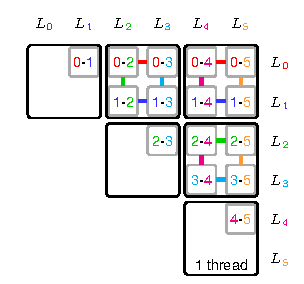
\includegraphics{embedsom/pic/reg-caching.pdf}
\caption{Detail of the caching of landmark data in \alg{Registers} projection kernel. Multiple landmark pairs (small boxes) are processed by each thread (large boxes). Caching of the landmark data in registers allows the reuse of loaded data (color lines), thus reducing the amount of memory accesses.}
\label{fig:proj}
\end{figure}

To further improve the data caching, we implemented algorithm \Alg{Registers}, where each thread computes more than one landmark pair in a single iteration so that the coordinates loaded into its registers can be shared as inputs among multiple landmark-pairs computations.
The data sharing scheme is detailed in Figure~\ref{fig:proj}.
We found that it is optimal to group the threads into small blocks of $2\times2$ computation items, saving half of the data loads.
Larger groups are theoretically possible, but even $3\times3$ caused excessive registry pressure and impaired performance on contemporary GPUs.
The innermost loop of the algorithm iterates over $d$ so that only a single \texttt{float4} value per each landmark is kept in registers.


\section{Experimental Results}\label{sec:results}

The main objective of the benchmarking was to measure the speedups achieved by different applied optimizations and to determine the optimal algorithms and their parameter setting for the sub-tasks of EmbedSOM computation.

The timing results, presented in the following sections, were collected as kernel execution times measured by a standard system high-precision clock. Each test was repeated $10\times$ and the mean values are presented in the subsequent figures. The relative standard deviations of the measurements were less than $5\%$ so we chose not to include them. Complete measurements are available in our GitHub repository\footnote{\url{https://github.com/asmelko/gpgpu24-artifact}}.

Results were collected on NVIDIA Tesla A100~PCIe~80~GB running CUDA 12.2. All benchmarking datasets were synthetic, containing exactly $1$Mi points ($n=2^{20}$, reflecting the common sizing of real-world datasets~\cite{adan2017flow}) with all coordinates sampled randomly from the same uniform distribution.
The performance of the benchmarked algorithms is not data-dependent, except for the case of caching performance in the projection step, where the completely random dataset is the worst-case scenario.


\subsection{Performance of $k$-NN selection}\label{sec:knn-evaluation}

Here we give an overview of performance and viable parameter settings observed for the $k$-NN selection algorithms.

Notably, all algorithms for $k$-NN are affected by CUDA thread block sizing which affects warp scheduling and data reuse possibilities of the shared-memory cache.
We observed that the total thread block size of $256$ threads was either optimal or near to optimal for almost all tested configurations, except for \alg{GridInsert} that performed the best with $64$ threads for lower values of $d$ and $g$ parameters.

Parameters $w$ and $h$\footnote{Technically, parameter $h$ is determined by the thread block size divided by $w$, we thus optimize only $w$.} of the \alg{GridInsert} algorithm determine the ratio between data transfers and computations, but may also affect the pressure on the shared memory.
Empirical evaluation indicates that the algorithm performs the best when each parallel insertion sort is performed in a separate warp, so the code divergence in SIMT execution is prevented (i.e., $w$ is a multiple of $32$)
The optimal performance was observed for $w$ equal to $96$ or $128$; However, the speedup over $w=32$ is relatively low.

\begin{figure}
	\centering
	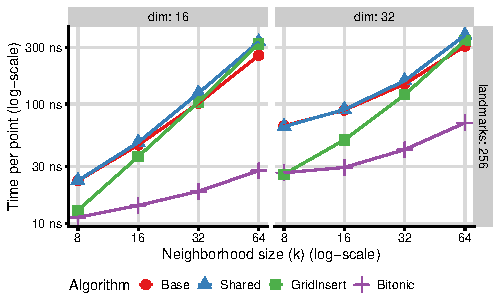
\includegraphics{embedsom/final-plots/algs_knn_repre_ampere.pdf}
	\caption{Amortized performance of $k$-NN step for a single input point using parameters usual in flow cytometry}
	\label{fig:knn-result-repre}
\end{figure}

A comparison of the best parametrizations of each algorithm on various configurations common in our target use cases is shown in Figure~\ref{fig:knn-result-repre}.
The \alg{Bitonic} algorithm significantly outperformed the other algorithms.
The speedup of \alg{Bitonic} over \alg{Base} was between $3\times$ to $20\times$ and usually more than $2\times$ over the second-ranking method.

The benchmarking also confirmed a rather huge scaling difference between algorithms based on divergent insertion sort and algorithms based on sub-quadratic parallelizable sorting schemes.
We conclude that despite the simplicity that might enable GPU speedups in certain situations, the insertion sort is too slow for larger values of $k$ in this case.

As an interesting result, we observed that despite following the general recommendations, the straightforward use of shared memory (in the \alg{Shared} algorithm) did not improve overall performance over the \alg{Base}.
Quite conversely, the overhead of explicit caching even caused a slight decrease in the overall performance.

% \begin{figure}
% 	\centering
% 	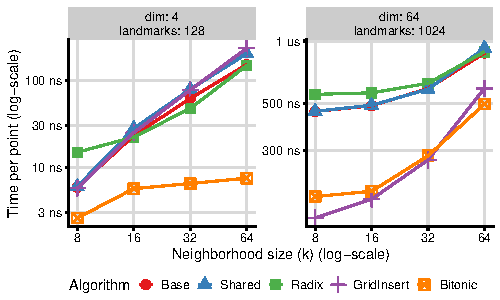
\includegraphics{embedsom/final-plots/algs_knn_extreme_ampere.pdf}
% 	\caption{Amortized $k$-NN step performance in corner-case parametrizations}
% 	\label{fig:knn-result-extreme}
% \end{figure}

We additionally report the performance measurements for two selected corner cases with extreme values of $g$ and $d$ (figure omitted due to the page limit).
Mainly, the total volume of the computation required to prepare the Euclidean distances scales with $g\cdot d$, which becomes dominant when both are maximized.
At that point, we observed that \alg{GridInsert} provides comparable or mildly better performance than \alg{Bitonic}, especially in cases where $k$ is small and the overhead of insertion sorting is not as pronounced.

Naturally, we should ask whether it could be feasible to combine the benchmarked benefits of \alg{GridInsert} and \alg{Bitonic} algorithms in order to get the best of both approaches (optimal inputs caching and fast $k$-NN filtering).
While an investigation of this possibility could be intriguing, we observed that a fused algorithm would require very complicated management of the shared memory (which both algorithms utilize heavily), and the estimated improvement of performance was not sufficient to substantiate this overhead; we thus left the question open for future research.


\subsection{Performance of projection step}

% \begin{figure}
% 	\centering
% 	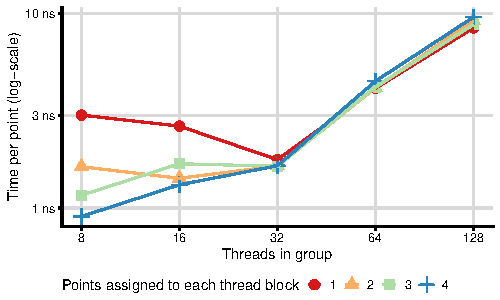
\includegraphics{embedsom/final-plots/proj_multi_block_ampere}
% 	\caption{Comparison of various sizes and numbers of thread groups in the \alg{Shared} projection algorithm in the extreme parametrization ($k = 8, d = 4$).}
% 	\label{fig:multi_block}
% \end{figure}

\begin{figure}
	\centering
	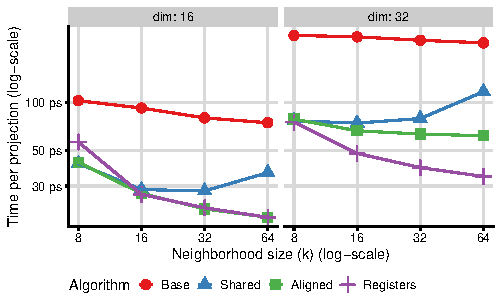
\includegraphics{embedsom/final-plots/algs_proj_repre_ampere}
	\caption{Amortized performance of a single projection operation in the algorithms that compute the projection step (showing the most important problem parametrizations)}
	\label{fig:proj_repre}
\end{figure}

The projection algorithms described in the previous section have only two execution parameters:
The size of the CUDA thread block and the number of data points assigned to a thread block (threads are divided among the points evenly).
We observed that selecting more than one point per thread block is beneficial only in the case of relatively small problem instances (low $k$ and $d$) because it prevents underutilization of the cores.

The optimal size of the CUDA thread blocks depends mainly on the parameters $k$ and $d$.
In case of \alg{Shared} algorithm, optimal values ranged from $32$ (for $k=8$, $d=4$) to $64$ ($k=d=64$).
With the caching optimizations in \alg{Aligned} and \alg{Registers}, the optimal thread block size was slightly higher, reaching $128$ for the most complex problem instances.
We assume this is a direct consequence of the improved memory access efficiency which gives space for parallel execution of additional arithmetic operations.

Figure~\ref{fig:proj_repre} shows the performance of the best algorithm configurations for the representative parametrizations.
All three algorithms perform almost equally for small $k$, giving around $3\times$ speedup over \alg{Base}.
The importance of optimizations in \alg{Aligned} and \alg{Registers} grows steadily when parameter $k$ increases, up to around $10\times$ speedup at $k=64$.
In conclusion, the optimal algorithm for the EmbedSOM projection is determined by the dimensionality of the dataset --- \alg{Registers} performs better at higher dimensions ($d\geq32$) while \alg{Aligned} was slightly better for lower dimensions.


\subsection{Complete algorithm}\label{sec:impl-complete}

A complete GPU implementation of the EmbedSOM algorithm is the combination of the best implementations of $k$-NN and projection steps.
The selected algorithms \alg{Bitonic} and \alg{Registers} are simply executed sequentially on large blocks of $X$, sharing only a single data exchange buffer for transferring the $k$-NN data.
Notably, since the data exchange between the algorithm parts is minimal, comprising only distances and neighbor indexes from the $k$-NN selection, we claim that no specific optimizations of the interface are required.

% Because of the relative complexity of the methods, we did not attempt to compute a theoretically possible data processing throughput.
% On the other hand, the collected results seem to scale proportionately to the asymptotic time complexities of the algorithms, roughly following $\mathcal{O}(n\cdot d\cdot g\cdot \log_2 k)$ for the $k$-NN and $\mathcal{O}(n\cdot d \cdot k^2)$ for the projection.
% That gives an optimistic outlook on the future scalability of the implementation, especially because the larger problem instances bear no additional overhead.

\begin{figure}
	\centering
	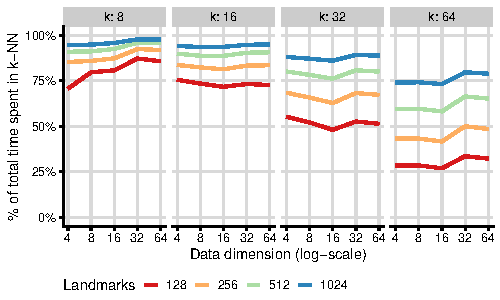
\includegraphics{embedsom/final-plots/esom_percent_ampere}
	\caption{The relative time spent by the $k$-NN computation usually dominates the execution of GPU EmbedSOM, composed of \alg{Bitonic}+\alg{Registers} algorithms.
  Projection computation time becomes dominant only for relatively impractical parametrizations of low $g$ and high $k$.}
	\label{fig:proj_percent}
\end{figure}

Finally, we highlight the relative computation complexity of both steps (Figure~\ref{fig:proj_percent}), which changes dynamically with $k$ and might be viable as a guide for further optimization.
We observed that for common parametrizations ($k\simeq 20$, $g\simeq 500$), most of the computation time is spent in $k$-NN step, and projection performance becomes problematic only in cases of almost impractically high $k$.
The results align with the asymptotic time complexities of the algorithms, roughly following $\mathcal{O}(n\cdot d\cdot g\cdot \log_2 k)$ for the $k$-NN and $\mathcal{O}(n\cdot d \cdot k^2)$ for the projection.

% The performance might be further improved by spatial indexing methods or approximate neighborhood selection algorithms, but we are currently not aware of a scheme that could provide a decisive performance improvement over the optimized brute-force neighbor processing~\cite{krulis2020detailed}.


\section{Related work}\label{sec:embedsom_relwork}

% In this work, we specifically reflect the needs of many areas of life sciences where large multidimensional point-cloud-like datasets occur, such as population biology, microscopy imaging, metagenomics, and others.

% Single-cell cytometry~\cite{adan2017flow} forms a canonical example of this niche: The recent development of hardware and measuring equipment has enabled a precise collection of multiple features of each of millions of cells in a sample. Clinicians and biologists commonly measure metrics such as protein expression on the cell surface using antibody-based markers. For instance, the marker detection may be performed optically by exciting fluorochromes with a laser and measuring emission spectra or using a specific binding of heavy metal ions detected by mass spectrometry techniques such as time-of-flight~\cite{spitzer2016mass}. Both methods allow cheap acquisition of data about more than 50 selected features at once, typically with several million single-cell measurements from each sample~\cite{vanikova2021omip,rodriguez2020systems}. Additionally, the development of single-cell sequencing methods has enabled to sequence the mRNA present in the individual cells~\cite{ziegenhain2017comparative}, typically yielding a dataset with thousands of data points of dimensions higher than $10^4$.

% Due to the variability in the samples, data, and measurements, analyzing and interpreting the results is challenging. Biologists usually analyze the datasets by linearly projecting the features to 2-dimensional plots and manually selecting the cells of interest in a process called gating~\cite{bashashati2009survey}. While computationally simple and easily interpretable by humans, gating gets extremely error-prone as the dimensionality of the dataset increases. It does not provide good support for detecting dataset features of dimensionality higher than $2$, such as complicated pathways and loops in cell phenotypes. Similarly, applying algorithms for clustering analysis provided good detection of cell phenotype clusters but minimal reliability in pathway-style feature detection~\cite{saelens2018comparison}.

% \begin{figure}
% \centering
% {\linewidth=21pc
% \begin{tikzpicture}[font=\tiny\sffamily\bfseries, inner sep=1pt]
% \node[inner sep=0, anchor=south west] (img) at (0,0) {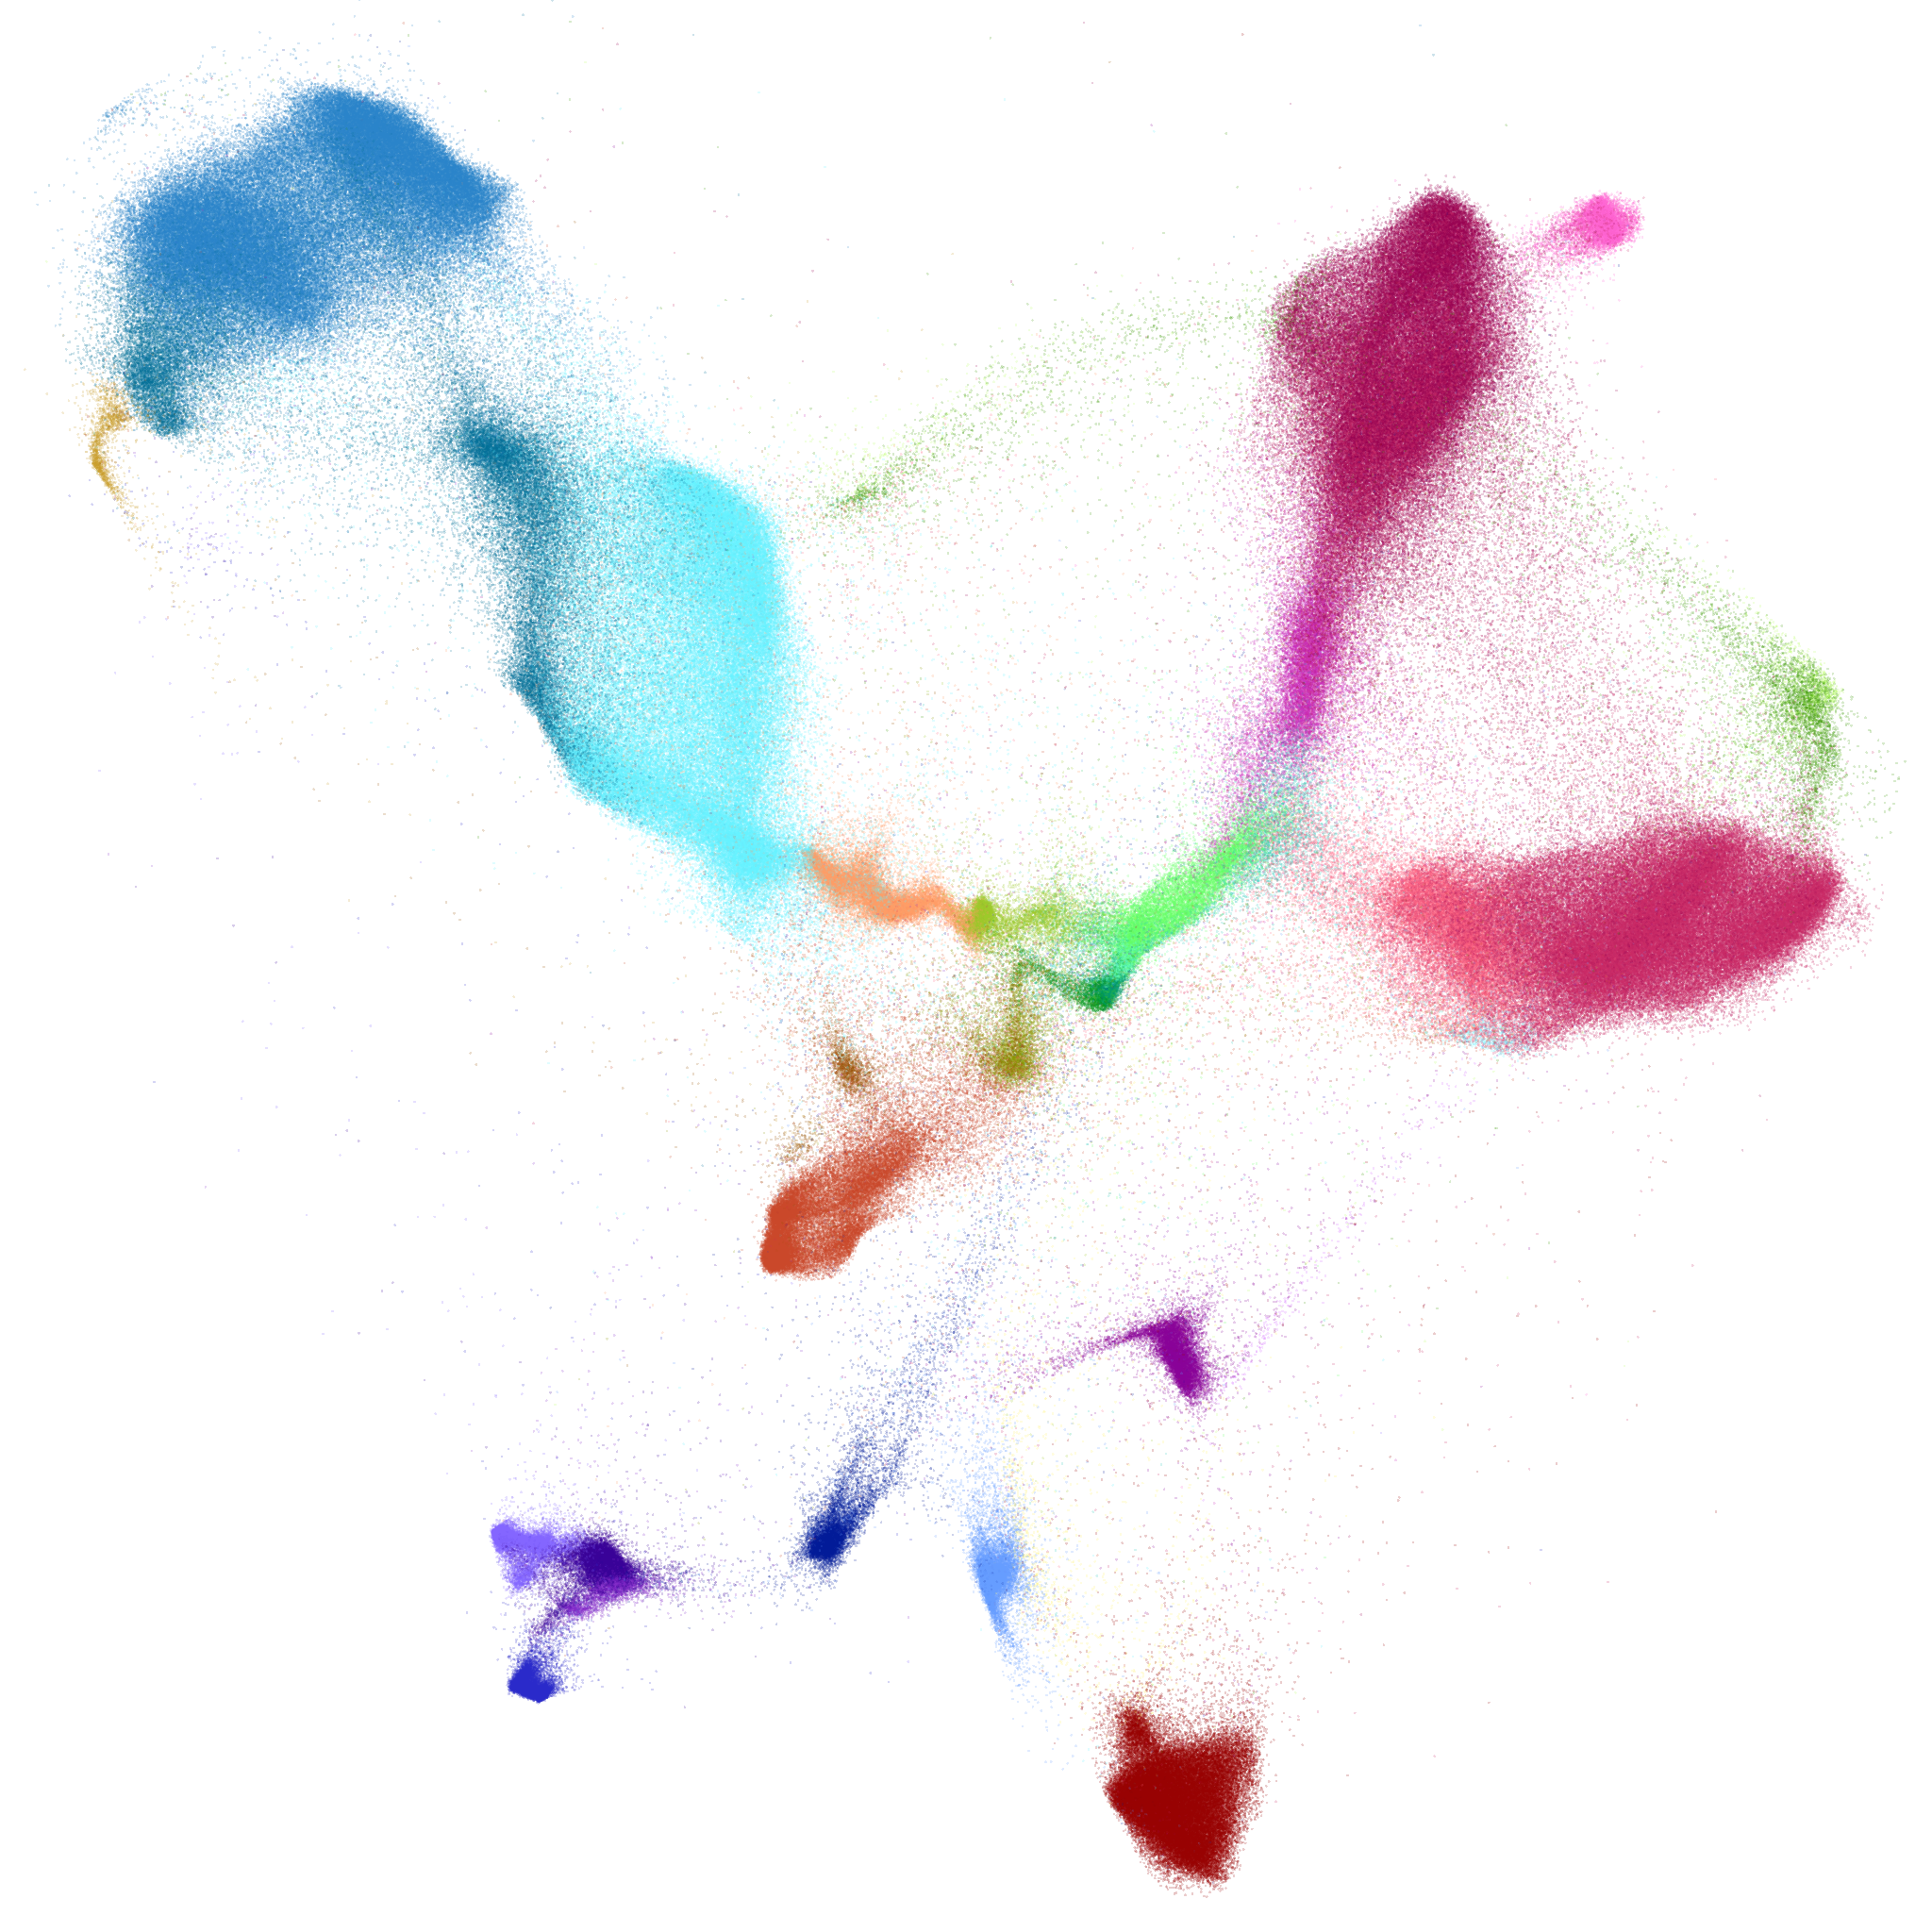
\includegraphics[width=\linewidth]{embedsom/pic/samusik-embedsom.png}};
% %\draw[help lines, xstep=0.1\linewidth, ystep=0.1\linewidth] (img.south west) grid (img.north east);
% \node[circle, draw] (A) at (0.5\linewidth,0.9\linewidth) {A};
% \node[circle, draw] (B) at (0.8\linewidth,0.2\linewidth) {B};
% \node[circle, draw] (C) at (0.2\linewidth,0.4\linewidth) {C};
% \node[circle, draw] (D) at (0.5\linewidth,0.266\linewidth) {D};
% \draw (A) to (0.45\linewidth,0.75\linewidth);
% \draw (A) to (0.9\linewidth,0.666\linewidth);
% \draw (B) to (0.55\linewidth,0.2\linewidth);
% \draw (B) to (0.65\linewidth,0.125\linewidth);
% \draw (B) to (0.55\linewidth,0.45\linewidth);
% \draw (C) to (0.5\linewidth,0.5\linewidth);
% \draw (C) to (0.275\linewidth,0.225\linewidth);
% \end{tikzpicture}}
% \caption{
% Example EmbedSOM projection of $841,644$ data points with $39$-dimensional single-cell measurements, representing the immune cell contents of bone marrow~\cite{samusik2016automated}. Colors were assigned manually to differentiate biologically relevant cell populations. Manual intervention in the unsupervised dimensionality reduction process would allow the user to fix several visualization deficiencies: overlapping pathways (labeled with~A), disconnected pathways (B), display of features in the small complex cell clusters (C), and the orientation and positioning of clusters that were chosen arbitrarily by the reduction process, not reflecting any biologically relevant features (D).
% }
% \label{fig:samusik}
% \end{figure}

% The development of non-linear dimensionality reduction algorithms in the last two decades has resolved many challenges. The new visualization-oriented methods, represented in the field mainly by t-SNE~\cite{maaten2008visualizing}, provided output that was sufficiently intuitive to understand, yet gave a satisfactory view of the highly complicated features that can not be observed by gating and projections. The tremendous success was quickly followed by new alternative algorithms that optimize different aspects of the process. UMAP~\cite{becht2019dimensionality} is currently a common choice for both visualization and a starting point of analysis, followed by PHATE~\cite{moon2019visualizing}, scvis\cite{ding2018interpretable}, TriMap\cite{amid2019trimap}, and others. For illustration, a typical example visualization is provided in~Figure~\ref{fig:samusik}, along with the description of common visualization problems.

% Following the plethora of newly introduced algorithms, a discussion unfolded to assess the optimality of the obtained visualization. Reviews have focused not only on reproducibility and robustness (i.e., susceptibility to significant changes in output caused by minor variations in data or different random seeds) but also on the representation of biologically valid features. Vast resources were invested into modifying the algorithms, especially t-SNE, to maximize various metrics, including convergence speed~\cite{belkina2019automated}, general performance~\cite{linderman2019fast}, robustness~\cite{polivcar2021embedding}, and the (very informally specified) quality of the display of local and global relations in data~\cite{kobak2019heavy,kobak2021initialization}. Some features required for high visualization quality are showcased in~Figure~\ref{fig:samusik}.

% User interaction possibilities in the dimensionality reduction process were therefore largely neglected, except for prohibitively small datasets where the use of force-based graph layouts and similar algorithms did not pose a throughput challenge. As one of few exceptions, van~Unen~et~al.~\cite{unen2017visual} and Chatzimparmpas~et~al.~\cite{chatzimparmpas2020t} achieved a methodological advance by extending the t-SNE algorithm, producing HSNE and t-viSNE respectively. HSNE organizes and visualizes a small data model dynamically using t-SNE, providing an intuitive way for the user to zoom into various compartments of the dataset, following a hierarchical structure of clusters. t-viSNE focuses on interactive use of t-SNE for exploration of complex dataset properties, but only of relatively small datasets.

% Compared to HSNE, our developments in BlosSOM provide two significant improvements: Full dataset may be rendered at all times (giving an unprecedented high-definition view of the features), which is enabled by a more efficient design of the base algorithm. Additionally, no hierarchical structure or no fixed layouting algorithm is imposed on the user, improving the display of structures that are hard to visualize or capture with hierarchical methods, such as the inter-cluster pathways.


% \subsection{GPU acceleration}

The essential component of our success is GPU acceleration of the projection computation which needs to be fast enough to re-calculate the embedding in real-time. 
In the following, we address the most relevant works that influenced or inspired our solution.

% One of the first GPU-accelerated dimensionality reduction methods was proposed in the work of Yeh et al.~\cite{yeh2010efficient} about twelve years ago. The first part uses $k$NN search with $k$-$d$-tree indexing structure. The GPU was used to compute Euclidean distances and to construct the tree using the radix sort algorithm. The projection itself used the Krylov subspace method for local linear embedding (LLE), which can be realized as a sparse matrix-vector multiplication so it was computed by cuBLAS. Despite the limited properties of the GPUs of the time, they were able to achieve $30$--$60\times$ speedup to the CPU implementation.

% A slightly different approach takes methods based on \emph{Principal Component Analysis} (PCA) algorithm. These methods are quite popular mainly since the principal components can be computed as eigenvectors of the data covariance matrix; thus, it can be implemented using linear algebra libraries. Martel et al.~\cite{martel2018implementation} proposed the implementation of PCA for CUDA and FPGAs. They have used the Jacobi method for the eigenvector decomposition, and the implementation heavily relied on Thrust and cuBLAS libraries. PCA is also used in more elaborate projection methods such as \emph{secant-based dimensionality reduction}~\cite{kvinge2018gpu}. The PCA is used to initialize a projection matrix, which is subsequently iteratively improved by a \emph{secant set} --- a set of normalized differences of all input point pairs. The projection matrix is multiplied with every secant to find a \emph{secant projection} with minimal $L_2$ norm. Although this method is theoretically intriguing, the GPU implementation is quite straightforward, using simple kernels and the cuSolver library.

Being one of the most profound visualization methods, \emph{t-SNE} was studied to explore the possibilities of having a fast GPU-enabled implementation. One of the initial implementations was t-SNE-CUDA library~\cite{chan2018t}. The most complicated step (computing the attractive forces of the N-body simulation) is handled as a multiplication of a sparse matrix and a vector by the CUSparse library. This work was slightly improved a year later \cite{chan2019gpu} when the authors replaced the CUSparse library with their implementation of multiplication, which takes advantage of atomic operations to perform the reduction in scalar sums.

% t-SNE can be improved by applying a hierarchical approach which can help both with the stability of the results and the computational demands of the algorithm. One of the first representatives that used a hierarchical approach and GPU acceleration was the Anchor-t-SNE (AtSNE) algorithm~\cite{fu2019atsne} which uses anchor points, selected representatives of the data which are projected first, and the remaining points are projected based on their proximity to the anchor points. A similar idea is used in the Barnes-Hut approximation of t-SNE\cite{van2014accelerating} which constructs a tree data structure that helps compute repulsive forces. This method was used in the work of Meyer et al.~\cite{meyer2020improving}, who implemented a warp-optimized CUDA version SWW-tSNE. Unlike the original t-SNE-CUDA, they have decided to use cuBLAS for the computation of attractive forces. The SWW-tSNE was later improved and accompanied with SWW-AtSNE~\cite{meyer2022global}, a warp-optimized version of anchor-based implementation of t-SNE~\cite{fu2019atsne}.

Perhaps the most popular contemporary method for data visualization is the \emph{Uniform Manifold Approximation and Projection} algorithm (UMAP), which often produces better results than t-SNE at the cost of higher computational demands. There are two GPU implementations worth mentioning which were both made part of RAPIDS cuML library~\cite{tegegne2021parallel, nolet2020bringing}. They both use a similar approach, implementing a kNN approximation based on gradient descent methods. The first implementation~\cite{tegegne2021parallel} relies more on existing solutions and libraries, and the second one~\cite{nolet2020bringing} is slightly more low-level as they implement the embedding using custom kernels.

Even though the presented methods (especially t-SNE) exceeded the speedup of two orders of magnitude, they are still quite far from real-time processing when the number of points reaches the order of millions. The proposed EmbedSOM projection is based on SOMs and linear projection based on $k$NN search~\cite{kratochvil2019generalized,kratochvil2020shinysom}, which is technically closest to the work of Yeh et al.~\cite{yeh2010efficient}. For the SOM part, we have adapted the state-of-the-art implementation of $k$-means algorithm~\cite{krulis2020detailed} since SOM shares many of its steps. The crucial part of the projection is the $k$NN search, which is also repeated in the aforementioned papers; however, we have found that the solution based on bitonic-sorting~\cite{krulivs2015optimizing} performs the best in our case.


\section{Conclusion}\label{sec:outro}

We have presented a GPU implementation for the semi-supervised dimensionality reduction algorithm EmbedSOM where we optimized independently two kernels: A general $k$NN search and a 2D projection which may be used independently. The $k$-NN was solved by adapted bitonic sorting, which eliminates thread divergence. The projection kernel was optimized to fetch and use data most efficiently by utilizing vector loads and data reuse on the register level. A thorough benchmarking indicates that both kernels achieved a significant speedup over the baseline GPU implementation.

The proposed implementation should enable subsequent research in interactive dimensionality reduction tools where the user changes SOM parameters or landmarks and the projections are re-computed and visualized in real-time. The results show that the optimized EmbedSOM version can project more than $1$ million individual data points each frame, while maintaining a frame rate above 30fps. 



% We have presented BlosSOM, a novel software for semi-supervised dimensionality reduction and visualization of large datasets.
% BlosSOM utilizes a GPU-accelerated implementation of the EmbedSOM algorithm as a highly efficient base for projecting the data to 2D, and improves its use with several supervision methods that allow the users to interactively and intuitively steer the process towards the desired solution with feedback.

% The GPU implementation in CUDA was thoroughly benchmarked and optimized.
% In BlosSOM, it is used to dynamically project the data points in an interactive visualization environment, where it re-projects and re-renders all data points every frame at high frame rate.
% On typical datasets, the optimized version is able to project more than 1 million of individual data points each frame, while maintaining a frame rate of 30fps or higher.

% We described and implemented several methods for user interaction with the landmark-based data model in EmbedSOM, based on self-organizing maps and graph embedding.
% The combination of the approaches in BlosSOM provided a solution to several challenges typically encountered with unsupervised dimensionality reduction.
% Finally, we demonstrated the use of BlosSOM on a biologically relevant use-case from single-cell cytometry, where it gives an effective way to produce desirable visualizations with variable level of details.

% We believe that the presented methodology will find use in explorative analysis of complex datasets, and provide a base for constructing intuitive, user-friendly annotation and dissection tools for single-cell cytometry data.

% \subsection{Data and software availability}\label{ssec:data}

% BlosSOM is available as free and open-source software from \texttt{https://github.com/\-molnsona/\-blossom}.
% Benchmark results are available from \texttt{https://github.com/\-asmelko/\-embed\-som-bench\-marks}.

% Datasets displayed in Sections \ref{sec:methods} and \ref{sec:results} are available from FlowRepository (\texttt{http://flow\-repository.org/\-id/FR-FCM-ZZPH}, file \texttt{Samusik\_all.fcs}) and from Smithsonian institute 3D digitization repository (\texttt{https://3d.si.edu/}, datasets `Mammuthus primigenius (Blumbach)' and `Tyrannosaurus rex', the 3D point coordinates were extracted manually from the vertex coordinates available in \texttt{.obj} files).


%%
%% The acknowledgments section is defined using the "acks" environment
%% (and NOT an unnumbered section). This ensures the proper
%% identification of the section in the article metadata, and the
%% consistent spelling of the heading.
% \begin{acks}
%   This paper was supported by Charles University institutional funding SVV 260698/2023.

% \end{acks}

